\documentclass{article}

\usepackage{graphicx}
\usepackage{fancyhdr}
\usepackage[sorting=none]{biblatex}
\usepackage[margin=1in]{geometry}
\usepackage{listings}
\usepackage[hidelinks]{hyperref}
\usepackage{xcolor}
\usepackage{xepersian}




\addbibresource{bibliography.bib}
\settextfont[Scale=1.2]{IRNazli.ttf}
\setlatintextfont[Scale=1]{times.ttf}
\renewcommand{\baselinestretch}{1.5}
\pagestyle{fancy}
\fancyhf{}
\renewcommand{\headrulewidth}{1pt}
\renewcommand{\footrulewidth}{1pt}
\setcounter{tocdepth}{1}
\begin{document}

\def\by{نگارش}
\def\superv{مدرس}
\def\faculty{دانشکده مهندسی کامپیوتر}
\def\course{رایانش عصبی}
\def\docTitle{پروژه دوم }
\def\supervisor{دکتر رضا صفابخش}
\def\fname{سیدمهدی }
\def\lname{میرفندرسکی}
\def\stuNum{401131065}
\def\docDate{آبان 1401}

\rhead{\docTitle}
\lhead{درس \course}
\rfoot{\fname \lname}
\lfoot{\stuNum}
\cfoot{\\ \thepage}



\begin{titlepage}
\begin{center}
%
\includegraphics[width=0.4\textwidth]{fa-logo.png}\\
\centerline{{
\includegraphics[height=3.8cm]{fa-logo}}}        
\LARGE
%\textbf{دانشگاه صنعتی اصفهان}\\
%\textbf{دانشکده مهندسی کامپیوتر}\\
\bf{\fontsize{16pt}{16pt}\selectfont دانشگاه صنعتی امیرکبیر}\par
\fontsize{14pt}{15pt}\selectfont(پلی‌تکنیک تهران)\par
\fontsize{16pt}{17pt}\selectfont \faculty \par
        
\par
        

\vfill
{\huge\settextfont{B_Titr.ttf}{\docTitle  درس  \course}}
\vfill
 
\settextfont[Scale=1.2]{BNazanin.ttf}
{\huge\by}\\
\fontsize{18pt}{19pt}\selectfont\bfseries{\fname \lname} \\
\settextfont[Scale=1.2]{BNazanin.ttf}
{\huge\superv}\\
{\fontsize{18pt}{19pt}\selectfont\bfseries\par\supervisor}\\
\fontsize{16pt}{17pt}\selectfont\docDate\\
 
 
        
\LARGE
%\textbf{نام و نام خانوادگی: مجید فرهادی}\\
%\textbf{شماره دانشجویی: 9700000}\\
%\textbf{نیم‌سال تحصیلی: پاییز 1400}\\
%\textbf{مدرّس: دکتر محمّدرضا حیدرپور}\\
%\textbf{دستیاران آموزشی: مجید فرهادی - دانیال مهرآیین - محمّد نعیمی}\\
\end{center}
\end{titlepage}


\tableofcontents

\newpage


% \begin{table}[h!]
%     \centering
%     \begin{tabular}{|c|c|c|l|l|l|l|}
%     \hline
%     \diag{مجموعه/}{\lr{epoch}}             & 10                       & 20 & 30 & 50  & 75 & 100 \\ \hline
%     صحت مجموعه آموزشی   & $0.92625$ & $0.9025$ & $0.90625$ & $0.938125$ & $0.94375$ & $0.981875$    \\ \hline
%     صحت مجموعه تست    & $0.9125$ & $0.8825$ & $0.8775$ & $0.91$ & $0.92$ & $0.98$    \\ \hline
%     \end{tabular}
% \end{table}

% \begin{figure}[!h]
%     \centering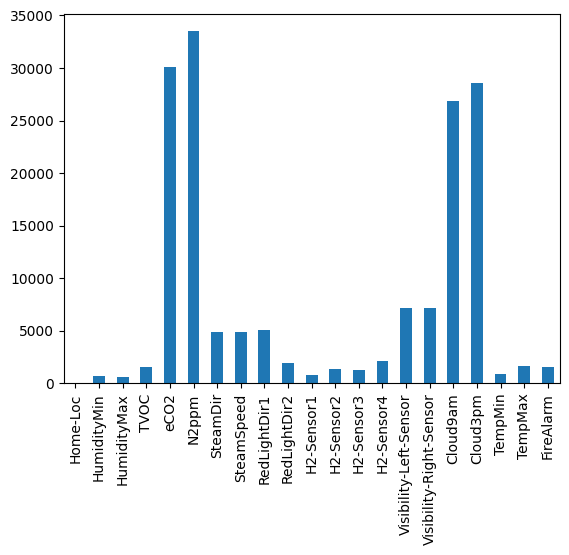
\includegraphics[scale=.45]{./p1-1}
%     \caption{پرسپترون نمودار 1}\label{fig.14}
% \end{figure}





\section{سوال اول}

\subsection{تخمین مقادیر گم‌شده}

روش‌های متعددی برای این قسمت وجود دارد که در ادامه به معرفی برخی از آن‌ها می‌پردازیم:

\begin{itemize}
    \item حذف سطر یا ستون‌ها: در این روش سطر و ستون‌هایی که شامل مقادیر گم‌شده هستند با شروطی می‌توانند حذف شوند.
    \item حذف سطر یا ستون‌هایی که درصد قابل توجهی از آن داده گم‌شده است.
    \item حذف یا نگهداری سطر یا ستون‌هایی که از یک مقدار حد آستانه بیشتر یا کمتر مقادیر گم‌شده دارند.
    \item همچنین می‌توان بر اساس زیر مجموعه‌ای از سطر یا ستون‌ها این مقادیر را حذف کرد.
    \item اما بعضی اوقات این مقادیر محدود هستند و ترجیح بر آن خواهد بود که سطرها یا ستون‌ها حذف نشوند. یک روش برای این کار پر کردن این مقادر با مقادیر ثابت خواهد بود که برای هر نوع داده‌ای می‌تواند مورد استفاده قرار گیرد.
    \item روش دیگر مورد استفاده برای پر کرده داده‌ها، استفاده از میانگین، میانه یا مد خواهد بود که می‌تواند مفید واقع شود.
    \item روش دیگر استفاده از مقدار قبلی یا بعدی در یک ستون مشخص است (مفید برای داده‌های سری زمانی).
\end{itemize}


\subsection{نرمال‌سازی}
\subsection{تبدیل ویژگی گسسته به عددی}
\subsection{حذف داده‌های پرت}
\subsection{تفکیک مجموعه داده}

\section{سوال دوم}


\section{سوال سوم}




\section{سوال چهارم}



\section{پیوست}

% \section{ضمیمه}
% برای آشنایی بیشتر با \lr{\LaTeX}، با جست‌و‌جو در اینترنت منابع مفیدی خواهید یافت.

% %\printbibliography[title=منابع]

% \section*{منابع}
% \renewcommand{\section}[2]{}%
% \begin{thebibliography}{99} % assumes less than 100 references
% %چنانچه مرجع فارسی نیز داشته باشید باید دستور فوق را فعال کنید و مراجع فارسی خود را بعد از این دستور وارد کنید

% \begin{LTRitems}

% \resetlatinfont

% % \bibitem{b1} http://mrheidar.ir/courses/operating\_system.html
% \end{LTRitems}

% \end{thebibliography}

\end{document}